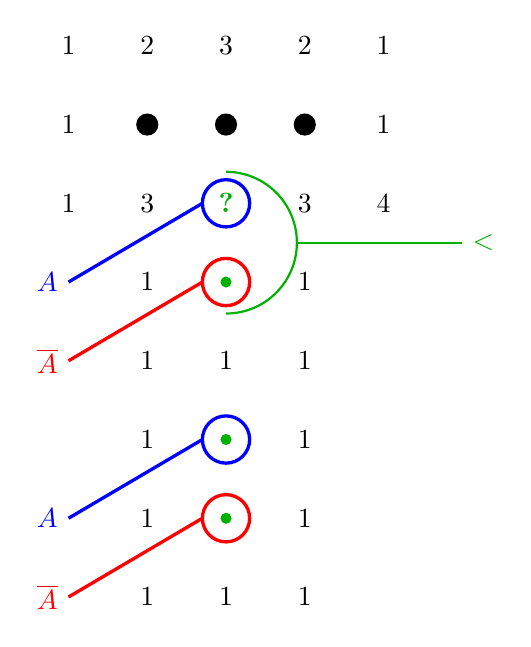
\begin{tikzpicture}
    \node at (0,0) {1};
    \node at (1,0) {2};
    \node at (2,0) {3};
    \node at (3,0) {2};
    \node at (4,0) {1};
    
    \node at (0,-1) {1};
    \fill (1,-1) circle (4pt);
    \fill (2,-1) circle (4pt);
    \fill (3,-1) circle (4pt);
    \node at (4,-1) {1};
    
    \node at (0,-2) {1};
    \node at (1,-2) {3};
    \node[color=green!70!black] at (2,-2) {\textbf{?}};
    \draw[blue, very thick] (2,-2) circle [radius=0.3] (1.7,-2) -- (0,-3) node[anchor=east] {\(A\)};
    \node at (3,-2) {3};
    \node at (4,-2) {4};


    \draw[thick, green!70!black] (2,-1.6) arc[start angle=90, end angle=-90, radius=0.9];
    
    \draw[thick, green!70!black](2.9,-2.5) -- (5,-2.5) node[anchor=west]{\(<\)};
    
    \node at (1,-3) {1};
    \fill[color=green!70!black] (2,-3) circle (2pt);
    \draw[red, very thick] (2,-3) circle [radius=0.3] (1.7,-3) -- (0,-4) node[anchor=east] {\(\overline A\)};
    \node at (3,-3) {1};
    
    \node at (1,-4) {1};
    \node at (2,-4) {1};
    \node at (3,-4) {1};

    \node at (1,-5) {1};
    \fill[color=green!70!black] (2,-5) circle (2pt);
    \draw[blue, very thick] (2,-5) circle [radius=0.3] (1.7,-5) -- (0,-6) node[anchor=east] {\(A\)};
    \node at (3,-5) {1};

    \node at (1,-6) {1};
    \fill[color=green!70!black] (2,-6) circle (2pt);
    \draw[red, very thick] (2,-6) circle [radius=0.3] (1.7,-6) -- (0,-7) node[anchor=east] {\(\overline A\)};
    \node at (3,-6) {1};

    \node at (1,-7) {1};
    \node at (2,-7) {1};
    \node at (3,-7) {1};
\end{tikzpicture}